\newcommand{\NWtarget}[2]{#2}
\newcommand{\NWlink}[2]{#2}
\newcommand{\NWtxtMacroDefBy}{Fragment defined by}
\newcommand{\NWtxtMacroRefIn}{Fragment referenced in}
\newcommand{\NWtxtMacroNoRef}{Fragment never referenced}
\newcommand{\NWtxtDefBy}{Defined by}
\newcommand{\NWtxtRefIn}{Referenced in}
\newcommand{\NWtxtNoRef}{Not referenced}
\newcommand{\NWtxtFileDefBy}{File defined by}
\newcommand{\NWtxtIdentsUsed}{Uses:}
\newcommand{\NWtxtIdentsNotUsed}{Never used}
\newcommand{\NWtxtIdentsDefed}{Defines:}
\newcommand{\NWsep}{${\diamond}$}
\newcommand{\NWnotglobal}{(not defined globally)}
\newcommand{\NWuseHyperlinks}{}
\documentclass{article}

% Кодировки и языковые пакеты
\usepackage[T2A]{fontenc}  % Поддержка кириллического шрифта
\usepackage[utf8]{inputenc}  % Кодировка UTF-8 для ввода
\usepackage[russian]{babel}  % Поддержка русского языка

% Настройка абзацев и отступов
\usepackage{indentfirst}  % Отступ первого абзаца в разделе
\usepackage{parskip}  % Управление интервалами между абзацами
\setlength{\parindent}{1.25em}  % Отступ абзаца
\setlength{\parskip}{0em}  % Отступ между абзацами

% Для создания таблиц и их форматирования
\usepackage{tabularx}  % Автоматическая регулировка ширины колонок
\usepackage{geometry}  % Установка полей документа
\geometry{left=30mm, top=20mm, right=15mm, bottom=20mm}  % Установка полей документа

% Работа с вербатимными окружениями и гиперссылками
\usepackage{fancyvrb}  % Расширенные возможности для вербатимного текста
\usepackage[colorlinks=true, linkcolor=black, urlcolor=black, citecolor=black, linktoc=all]{hyperref}  % Создание гиперссылок в документе
\usepackage{comment}

% Форматирование заголовков и секций
\usepackage{titlesec}  % Настройка стиля заголовков разделов
\titleformat{\section}[block]{\Large\bfseries\filcenter}{}{1em}{}  % Формат заголовков разделов

% Для добавления кода и математики
\usepackage{listings}  % Вставка кода с подсветкой синтаксиса
\usepackage{amsmath}  % Дополнительные математические символы и окружения
\usepackage{amssymb} % Для использования \blacksquare

% Для создания графиков и визуализации данных
\usepackage{pgfplots}  % Построение графиков

% Библиография
\usepackage[style=numeric,sorting=nyt]{biblatex} % Создание библиографии
\addbibresource{book.bib}  % Указание файла с библиографией
\usepackage{tocbibind}% Пакет для автоматического добавления библиографии в содержание с нумерацией

\usepackage[strings]{underscore} % Позволяет спокойно юзать "_"




\title{Отчет о разработке программы, имитирующей случайные блуждания в графе}
\author{Пелагеев Д.И.}
\date{\today}

\begin{document}
\maketitle
\newpage
\tableofcontents
\newpage

\section{Введение}
Цель данной работы – это изучить применения теории графов для моделирования и анализа электрических цепей, представленных в виде графов, а также определение среднего времени перемещения между двумя вершинами графа с использованием метода случайного блуждания. Мы рассматриваем однородное случайное блуждание, при котором каждая вершина выбирает одну из своих соседних вершин с равной вероятностью на каждом шаге.

Электрические сети могут быть эффективно представлены с помощью графов, где вершины соответствуют узлам сети, а ребра — проводникам или линиям связи между этими узлами. Одним из ключевых аспектов анализа таких сетей является расчет сопротивления между двумя узлами, что имеет важное значение для оценки характеристик сети и её надежности. Этот расчет можно провести с использованием законов Кирхгофа, но альтернативный подход предполагает использование методов теории графов и случайного блуждания.

В данной работе мы реализуем метод моделирования случайного блуждания по графу для вычисления среднего времени посещения указанной вершины и среднего времени обхода всего графа. Этот метод основывается на предположении, что время перемещения по каждому ребру равно единице, а выбор следующей вершины происходит случайно с равной вероятностью для всех соседей текущей вершины. Интересным является тот факт, что среднее время перемещения тесно связано с электрическим сопротивлением между узлами графа, если сопротивление каждого ребра также принять равным единице.

В данном отчете была разработана программа на Octave, которая имитирует случайные блуждания.
\newpage

\section{Теоретические основы}

\subsection{Основные понятия теории графов}

Теория графов, изучает графы - абстрактные структуры, состоящие из вершин (узлов) и рёбер (связей между узлами). Основные понятия теории графов включают следующие элементы:

Граф \(G = (V, E)\) состоит из множества вершин \(V\) и множества рёбер \(E\), где каждое ребро представляет собой пару вершин. Граф может быть ориентированным (если рёбра имеют направление) и неориентированным (если рёбра не имеют направления).

Матрица смежности \(A\) графа \(G\) размером \(n \times n\) (где \(|V|\) обозначает количество вершин графа и равна \(n\) задается как квадратная матрица, в которой элемент \(a_{ij}\) равен 1, если существует ребро между вершинами \(v_i\) и \(v_j\), и 0 в противном случае. И где \(\) Для ориентированного графа матрица смежности не обязательно симметрична\cite{7}.

Степень вершины \(v\) в графе \(G\) (обозначаемая как \(\deg(v)\)) - это количество рёбер, связанных с данной вершиной. В ориентированном графе различают входящую степень (\(\deg_{in}(v)\)) и исходящую степень (\(\deg_{out}(v)\))\cite{6}.

Граф \(G\) называется связным, если существует путь между любой парой вершин. Для ориентированных графов используется понятие сильной связности, когда для любой пары вершин \(u\) и \(v\) существует ориентированный путь как от \(u\) к \(v\), так и от \(v\) к \(u\)\cite{8}.

\subsection{Связь между случайными блужданиями и электрическими сопротивлениями}

Случайное блуждание на графе \(G\) представляет собой процесс, при котором на каждом шаге изменяется состояние случайного процесса, заключающееся в перемещении из текущей вершины в одну из соседних вершин, выбранную независимым образом с равной вероятностью. Этот процесс можно моделировать с помощью матрицы переходов \(P\), где элемент \(p_{ij}\) представляет собой вероятность перехода из вершины \(v_i\) в вершину \(v_j\).

Электрические сети могут быть представлены в виде графов, где вершины соответствуют узлам сети, а рёбра - проводникам или линиям связи. Для анализа таких сетей используется подход основаный на теории графов и модели случайных блужданий.

Сопротивление между двумя узлами \(i\) и \(j\) в электрической сети можно вычислить, моделируя сеть в виде графа и используя случайные блуждания. В частности, среднее время первого попадания из узла \(i\) в узел \(j\) тесно связано с электрическим сопротивлением между этими узлами.

Для расчета среднего времени первого попадания (hitting time) можно использовать следующюю формулу. Пусть \(G\) - граф, где \(V\) - множество вершин, \(E\) - множество рёбер. Рассмотрим однородное случайное блуждание, при котором вероятность перехода из одной вершины в любую соседнюю вершину, одинакова и равно к \(1/d(j)\). А среднее время случайного перемещения из \(i\) в \(j\) и обратно (commute time) будет тогда  равно \(1/d(j) + 1/d(i)\), где \(d(x)\) - степень вершины \(x\). 

\clearpage
\subsection{Время первого попадания}
\subsubsection{Теорема 1. О времени первого попадания}

Среднее время первого попадания в вершину \(j\) из вершины \(i\) определяется как разность потенциалов в Сценарии A:

$$\phi_{ij} = H_{ij}  \eqno(1)$$

\begin{figure}[h]
    \centering
    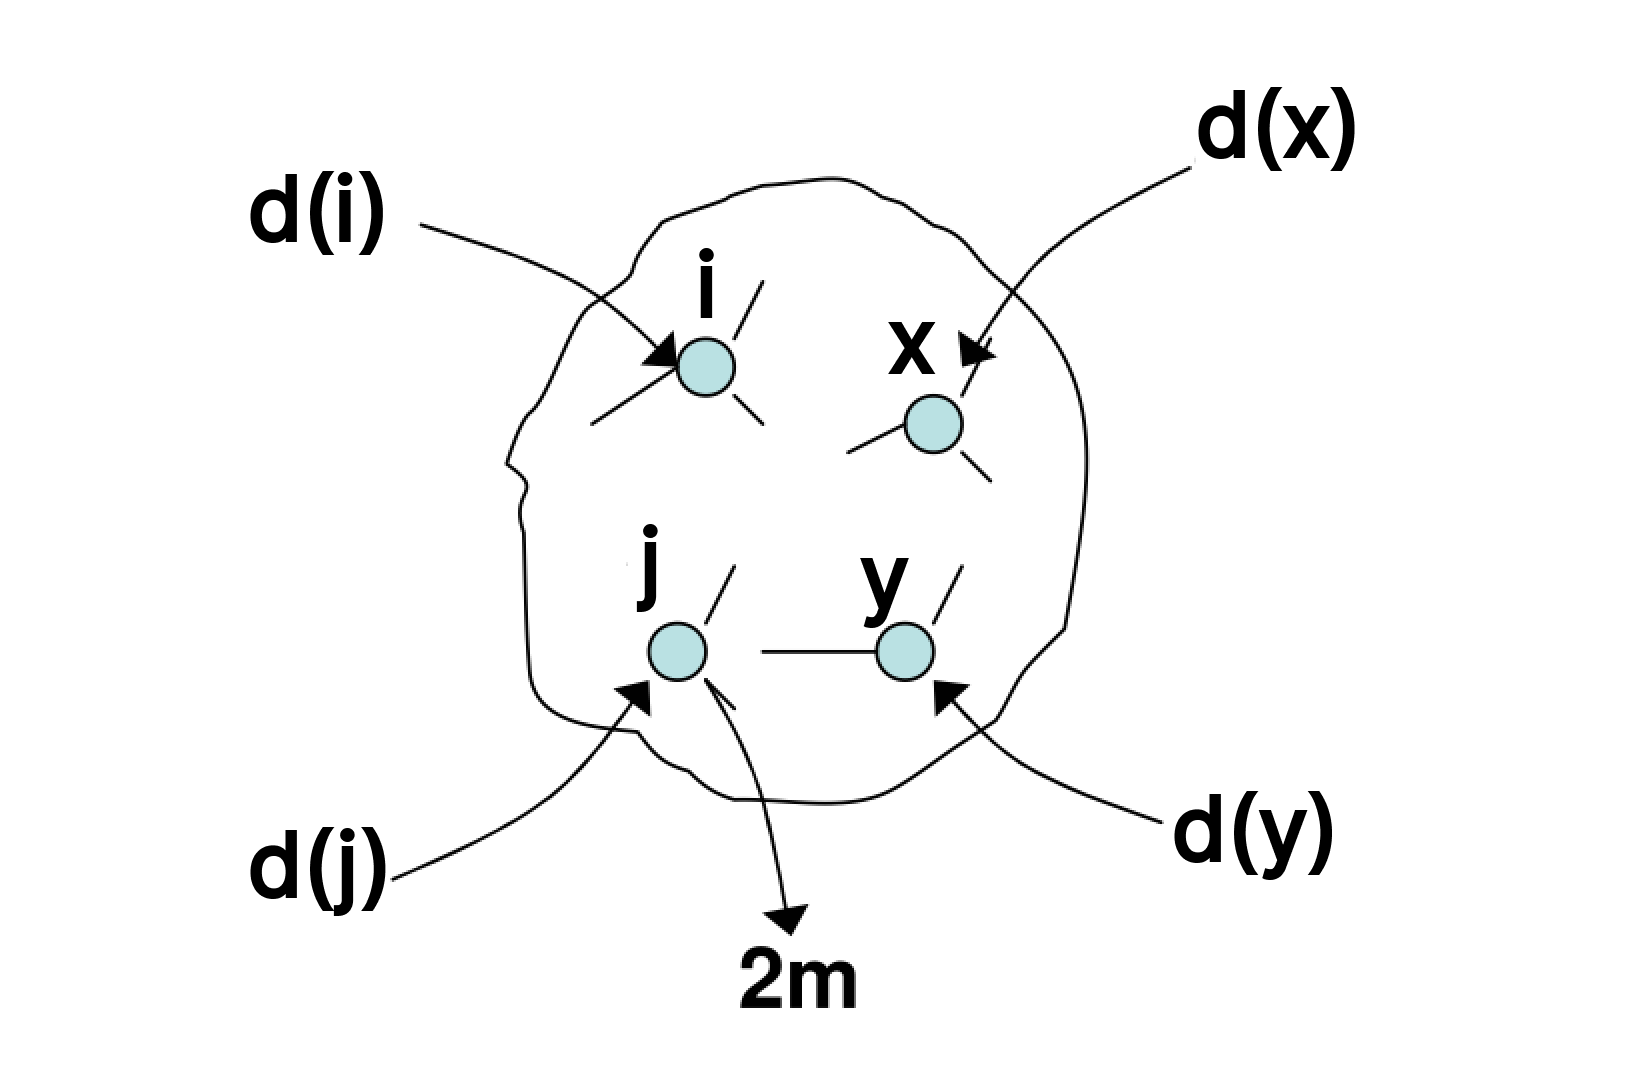
\includegraphics[width=0.3\linewidth]{A.png}
    \caption{Сценарий A}
    \label{fig:your_label}
\end{figure}

Теорема взята из \cite{1}, лемма 24.6.

\subsubsection{Доказательство}

Для доказательства данной теоремы введем законы Кирхгофа и Ома:

\begin{itemize}
    \item Суммарный ток в вершине и из нее равен нулю (K1) \cite{4}
    \item Сумма разностей потенциалов в любом цикле равна нулю (K2) \cite{4}
    \item Ток, протекающий по любому ребру, равен \(\frac{\text{разности потенциалов}}{\text{сопротивление}}\) (Закон Ома) \cite{5}
\end{itemize}


Теперь рассмотрим любую вершину \(i \in V\) . Используя законы Кирхгофа и Ома, мы имеем:

$$d(i) = \sum_{(i, x) \in E} \text{текущая } i \to x  \text{(K1)} $$
$$= \sum_{(i, x) \in E} \phi_{ix}   \text{(Закон Ома)} $$
$$= \sum_{(i, x) \in E} (\phi_{ij} - \phi_{xj}) \text{(K2)} $$
$$= d(i)\phi_{ij} - \sum_{(i, x) \in E} \phi_{xj} $$

Преобразование даст:

$$
\phi_{ij} = 
\begin{cases} 
0 &  i = j \\
1 + \frac{1}{d(i)} \sum\limits_{(i,x) \in E} \phi_{xj} &  i \neq j
\end{cases} 
\eqno(2)
$$


С другой стороны, рассмотрим случайную прогулку, начинающуюся с \(i\). Рассматривая только первый шаг этой прогулки, мы видим, что время попадания \(H_{uv}\) удовлетворяет следующим условиям:

$$
H_{ij} = 
\begin{cases} 
0 &  i = j \\
1 + \frac{1}{d(i)} \sum\limits_{(i,x) \in E} H_{xj} &  i \neq j
\end{cases} 
\eqno(3)
$$

Но это точно такая же система линейных уравнений, как и (2), удовлетворяемая \(\phi_{ij}\). Поскольку мы знаем, что эта система имеет единственное решение (потенциалы однозначно определяются потоками тока), мы выводим, что:

$$H_{ij} =  \phi_{ij}  \quad \forall i \in V  $$
\begin{flushright}
    \(\blacksquare\)
\end{flushright}

\subsection{Эффективное сопротивление}

Эффективное сопротивление (резистивное расстояние) \(\Omega_{vw}(\mathcal{L})\) между вершинами \(u\) и \(v\) в графе с равным сопротивлением \(r\) на всех рёбрах определяется как сумма взвешенных квадратов разностей между компонентами собственных векторов графа для всех пар узлов \(v\) и \(w\). В частности, для каждого узла \(v\) и \(w\) вычисляется разность компонент собственных векторов \(\psi_{jv}\) и \(\psi_{jw}\), которые соответствуют ненулевым собственным значениям \(\lambda_j(\mathcal{L})\) лапласиана. Затем, каждая разность возводится в квадрат, делится на соответствующее собственное значение, и все такие дроби суммируются для всех j от 2 до n. :

$$ \Omega_{vw}(\mathcal{L}) = \sum_{j=2}^{n} \frac{1}{\lambda_j(\mathcal{L})} (\psi_{jv} - \psi_{jw})^2 \eqno(4.1)$$


Данная запись присутствует в \cite{2} на стр. 11, но для  удобства, формула (4.1) будет видоизменена:


$$ R_{ij} = \sum_{k=1}^{n-1} \frac{(u_{ki} - u_{kj})^2}{\lambda_k} \eqno(4.2)$$


В формуле 4.2 \(\lambda_k\) – это собственные значения Лапласиана, где \(\lambda_0 = 0\), \(u_{ki}\) и \(u_{kj}\) - i-я и j-я компоненты k-го собственного вектора Лапласиана, а n – это вершины. Лапласиан, или матрица Лапласа определяется как матрица степеней \(D\) минус матрица смежности \(A\):
$$  \mathcal{L} = D - A  $$


\subsection{Время возвращения}
\subsubsection{Теорема 2. О времени возвращения}
Среднее время случайного перемещения из i в j и обратно определяется как cреднее время первого попадания в вершину \(j\) из вершины \(i\) плюс cреднее время первого попадания в вершину \(i\) из вершины \(j\) иле же как количество ребер \(m\) умноженное на эффективное сопротивление \(R_{ij}\) умноженное на два.

$$ C_{ij} = H_{ij} + H_{ji} = 2mR_{ij}\eqno(5)$$

Формула взята из \cite{3}, стр. 577.

\subsubsection{Доказательство}

Для доказательства используем сценарий B, который похож на сценарий A, за исключением того, что мы удаляем \(2m\) единиц тока с узла \(i\), а не с узла \(j\). Обозначая разность потенциалов в сценарии B через \(\phi^{'}\), мы имеем, согласно теореме 1:
$$\phi_{ji}^{'} = H_{ji} \eqno(6)$$

Теперь рассмотрим сценарий C, который похож на сценарий B, но с обратными токами. Обозначив разность потенциалов
обозначив разность потенциалов в этом сценарии через  \(\phi^{''}\), мы получим:

$$\phi_{ij}^{''} = \phi_{ji}^{'} = H_{ji} \eqno(7)$$

\begin{figure}[h]
    \centering
    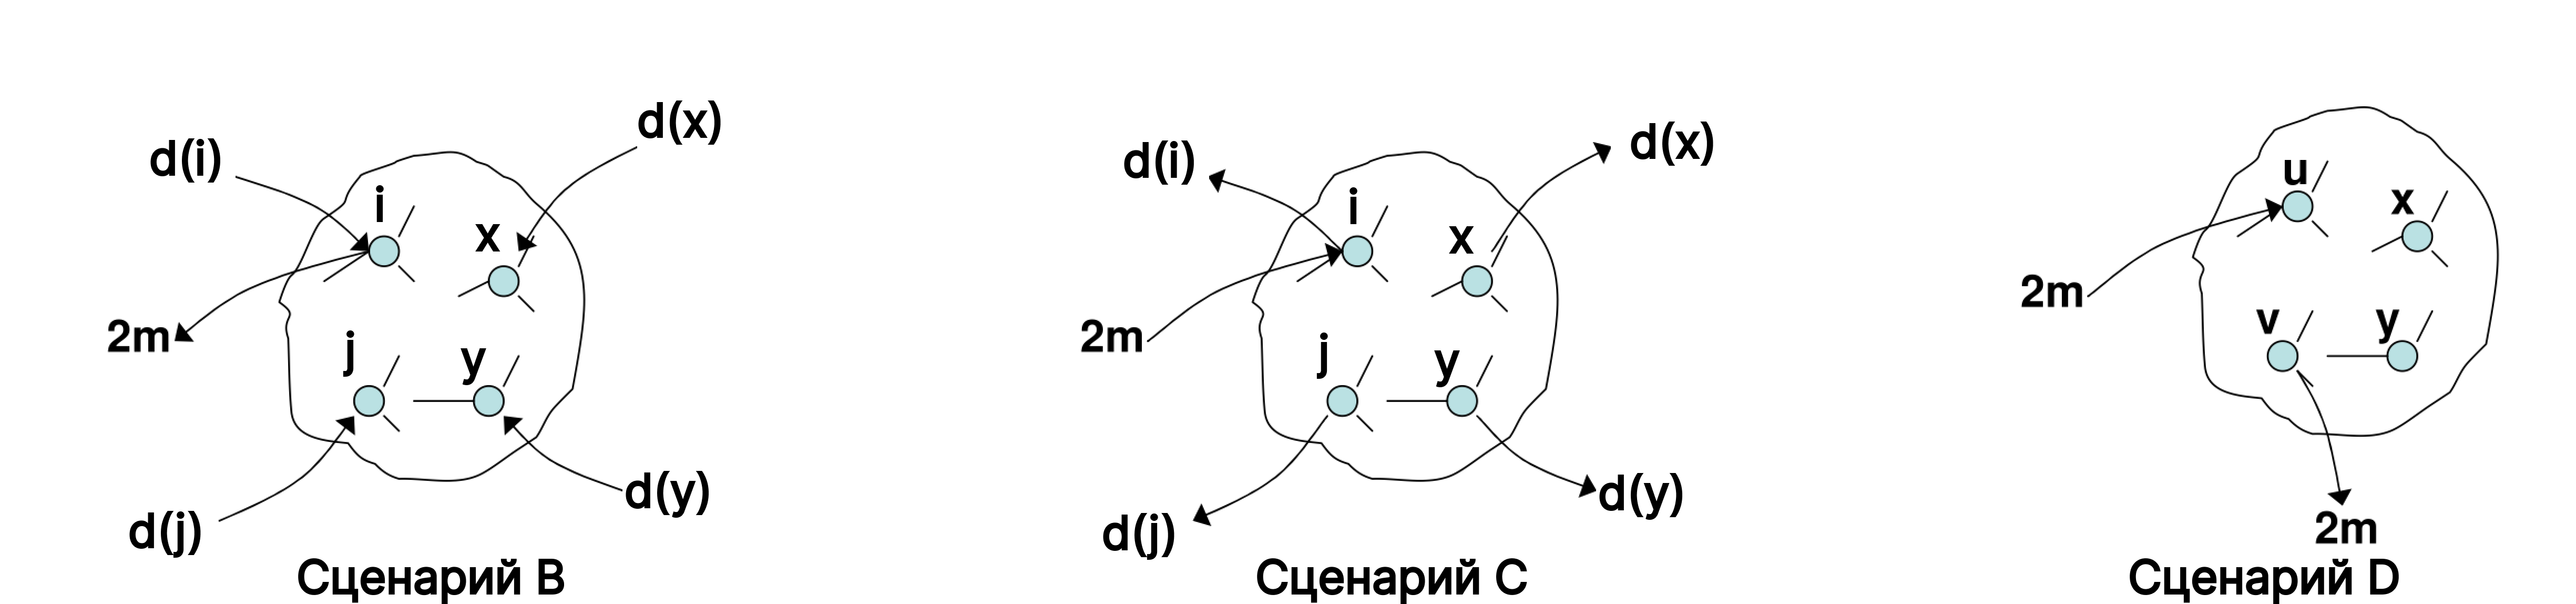
\includegraphics[width=1\linewidth]{BCD.png}
    \caption{Сценарий B,C и D}
    \label{fig:your_label}
\end{figure}

Наконец, рассмотрим сценарий D, который представляет собой сумму сценариев A и C. В силу линейности и обозначения потенциальные различия в сценарии D через \(\phi^{'''}\), мы имеем:

$$\phi_{ij}^{'''} = \phi_{ij} + \phi_{ij}^{''}= H_{ij} = H_{ji} \eqno(8)$$

Так как \(\phi_{ij}^{''}\) – это разность потенциалов, необходимая для перемещения \(2m\) единиц тока из \(i\) в \(j\), поэтому по закону Ома она равна \(2mR_{ij}\).



\section{Реализация программы}


\subsection{Переменные}
\subsubsection{Входные переменные}

\begin{itemize}
    \item \texttt{adj} - матрица смежности графа.
    \item \texttt{start} - индекс начального узла.
    \item \texttt{end_} - индекс конечного узла.
    \item \texttt{num_sim} - количество симуляций.
\end{itemize}

\subsubsection{Выходные переменные}

\begin{itemize}
    \item \texttt{fht} - вектор, содержащий время первого попадания в конечный узел для каждой симуляции.
    \item \texttt{ct} - вектор, содержащий время полного обхода графа для каждой симуляции.
    \item \texttt{cmt} - вектор, содержащий время перемещения от начального узла к конечному и обратно для каждой симуляции.
    \item \texttt{sfh} - отсортированный вектор времени первого попадания и их количества.
    \item \texttt{sct} - отсортированный вектор времени полного обхода графа и их количества.
    \item \texttt{scmt} - отсортированный вектор времени перемещения и их количества.
    \item \texttt{mfht} - среднее время первого попадания в конечный узел.
    \item \texttt{mct} - среднее время полного обхода графа.
    \item \texttt{mcmt} - среднее время перемещения от начального узла к конечному и обратно.
    \item \texttt{eff_res} - эффективное сопротивление графа, рассчитанное как среднее время перемещения, деленное на удвоенное количество ребер.
\end{itemize}

\subsubsection{Промежуточные переменные}

\begin{itemize}
    \item \texttt{n} - количество узлов в графе.
    \item \texttt{m} - количество ребер в графе, рассчитанное как половина суммы всех элементов матрицы смежности.
    \item \texttt{curr} - текущий узел в процессе блуждания.
    \item \texttt{visited} - булевый вектор, указывающий, были ли посещены узлы.
    \item \texttt{steps} - количество шагов, сделанных в текущей симуляции.
    \item \texttt{first_hit} - булева переменная, указывающая, было ли достигнуто первое попадание в конечный узел.
    \item \texttt{visit_count} - количество посещенных узлов.
    \item \texttt{neighbors} - вектор соседних узлов для текущего узла.
    \item \texttt{next} - следующий узел для перехода.
    \item \texttt{cms} - количество шагов для перемещения от начального узла к конечному и обратно в текущей симуляции.
    \item \texttt{file_path} - путь к файлу с матрицей смежности.
    \item \texttt{elapsed_time} - время, затраченное на выполнение симуляций.
\end{itemize}

\subsection{Скрипт random_walk.m}
В данной работе была разработана программа на языке Octave, которая имитирует случайные блуждания по графу, заданному матрицей смежности. Программа рассчитывает статистические данные. Об этих данных ниже рассказано более подробно. 


\begin{flushleft} \small
\begin{minipage}{\linewidth}\label{scrap1}\raggedright\small
\NWtarget{nuweb8a}{} $\langle\,${\itshape random_walk}\nobreak\ {\footnotesize {8a}}$\,\rangle\equiv$
\vspace{-1ex}
\begin{list}{}{} \item
\mbox{}\verb@@\\
\mbox{}\verb@function [fht, ct, sfh, sct, mfht, mct, eff_res, ...@\\
\mbox{}\verb@mcmt, scmt] = random_walk(adj, start, end_, num_sim)@\\
\mbox{}\verb@@\hbox{$\langle\,${\itshape initialization of variables}\nobreak\ {\footnotesize \NWlink{nuweb8c}{8c}}$\,\rangle$}\verb@@\\
\mbox{}\verb@@\hbox{$\langle\,${\itshape simulation loop}\nobreak\ {\footnotesize \NWlink{nuweb8d}{8d}}$\,\rangle$}\verb@@\\
\mbox{}\verb@@\hbox{$\langle\,${\itshape calculation}\nobreak\ {\footnotesize \NWlink{nuweb10b}{10b}}$\,\rangle$}\verb@@\\
\mbox{}\verb@@\hbox{$\langle\,${\itshape sort function}\nobreak\ {\footnotesize \NWlink{nuweb10c}{10c}}$\,\rangle$}\verb@@\\
\mbox{}\verb@@{\NWsep}
\end{list}
\vspace{-1.5ex}
\footnotesize
\begin{list}{}{\setlength{\itemsep}{-\parsep}\setlength{\itemindent}{-\leftmargin}}
\item \NWtxtMacroRefIn\ \NWlink{nuweb8b}{8b}.

\item{}
\end{list}
\end{minipage}\vspace{4ex}
\end{flushleft}
\begin{flushleft} \small
\begin{minipage}{\linewidth}\label{scrap2}\raggedright\small
\NWtarget{nuweb8b}{} \verb@"random_walk.oc"@\nobreak\ {\footnotesize {8b}}$\equiv$
\vspace{-1ex}
\begin{list}{}{} \item
\mbox{}\verb@@\hbox{$\langle\,${\itshape random_walk}\nobreak\ {\footnotesize \NWlink{nuweb8a}{8a}}$\,\rangle$}\verb@@{\NWsep}
\end{list}
\vspace{-1.5ex}
\footnotesize
\begin{list}{}{\setlength{\itemsep}{-\parsep}\setlength{\itemindent}{-\leftmargin}}

\item{}
\end{list}
\end{minipage}\vspace{4ex}
\end{flushleft}
В этом блоке инициализируются переменные для количества узлов и ребер в графе, векторов для хранения времени первого попадания, времени полного обхода, и времени перемещения.

\begin{flushleft} \small
\begin{minipage}{\linewidth}\label{scrap3}\raggedright\small
\NWtarget{nuweb8c}{} $\langle\,${\itshape initialization of variables}\nobreak\ {\footnotesize {8c}}$\,\rangle\equiv$
\vspace{-1ex}
\begin{list}{}{} \item
\mbox{}\verb@@\\
\mbox{}\verb@    n = size(adj, 1);@\\
\mbox{}\verb@    m = sum(adj(:)) / 2;@\\
\mbox{}\verb@    fht = zeros(num_sim, 1);@\\
\mbox{}\verb@    ct = zeros(num_sim, 1);@\\
\mbox{}\verb@    cmt = zeros(num_sim, 1);@\\
\mbox{}\verb@@{\NWsep}
\end{list}
\vspace{-1.5ex}
\footnotesize
\begin{list}{}{\setlength{\itemsep}{-\parsep}\setlength{\itemindent}{-\leftmargin}}
\item \NWtxtMacroRefIn\ \NWlink{nuweb8a}{8a}.

\item{}
\end{list}
\end{minipage}\vspace{4ex}
\end{flushleft}
Этот блок выполняет цикл по числу симуляций для выполнения случайных блужданий.

\begin{flushleft} \small
\begin{minipage}{\linewidth}\label{scrap4}\raggedright\small
\NWtarget{nuweb8d}{} $\langle\,${\itshape simulation loop}\nobreak\ {\footnotesize {8d}}$\,\rangle\equiv$
\vspace{-1ex}
\begin{list}{}{} \item
\mbox{}\verb@@\\
\mbox{}\verb@@\hbox{$\langle\,${\itshape initialising the current state}\nobreak\ {\footnotesize \NWlink{nuweb8e}{8e}}$\,\rangle$}\verb@@\\
\mbox{}\verb@@\hbox{$\langle\,${\itshape graph wandering cycle}\nobreak\ {\footnotesize \NWlink{nuweb9a}{9a}}$\,\rangle$}\verb@@\\
\mbox{}\verb@@\hbox{$\langle\,${\itshape hit check}\nobreak\ {\footnotesize \NWlink{nuweb9b}{9b}}$\,\rangle$}\verb@@\\
\mbox{}\verb@@\hbox{$\langle\,${\itshape update visited nodes}\nobreak\ {\footnotesize \NWlink{nuweb9c}{9c}}$\,\rangle$}\verb@@\\
\mbox{}\verb@@\hbox{$\langle\,${\itshape record round-trip time}\nobreak\ {\footnotesize \NWlink{nuweb9d}{9d}}$\,\rangle$}\verb@@\\
\mbox{}\verb@@\hbox{$\langle\,${\itshape calculation of travel time}\nobreak\ {\footnotesize \NWlink{nuweb10a}{10a}}$\,\rangle$}\verb@@\\
\mbox{}\verb@@{\NWsep}
\end{list}
\vspace{-1.5ex}
\footnotesize
\begin{list}{}{\setlength{\itemsep}{-\parsep}\setlength{\itemindent}{-\leftmargin}}
\item \NWtxtMacroRefIn\ \NWlink{nuweb8a}{8a}.

\item{}
\end{list}
\end{minipage}\vspace{4ex}
\end{flushleft}
Этот блок начинает наш основной цикл, инициализируюя текущий узел как начальный узел , а также массивы для отслеживания посещенных узлов и количества шагов. Также инициализируются переменные для отслеживания первого попадания в конечный узел и количества посещенных узлов.

\begin{flushleft} \small
\begin{minipage}{\linewidth}\label{scrap5}\raggedright\small
\NWtarget{nuweb8e}{} $\langle\,${\itshape initialising the current state}\nobreak\ {\footnotesize {8e}}$\,\rangle\equiv$
\vspace{-1ex}
\begin{list}{}{} \item
\mbox{}\verb@@\\
\mbox{}\verb@    for sim = 1:num_sim@\\
\mbox{}\verb@        curr = start;@\\
\mbox{}\verb@        visited = false(n, 1);@\\
\mbox{}\verb@        visited(start) = true;@\\
\mbox{}\verb@        steps = 0;@\\
\mbox{}\verb@        first_hit = false;@\\
\mbox{}\verb@        visit_count = 1;@\\
\mbox{}\verb@@{\NWsep}
\end{list}
\vspace{-1.5ex}
\footnotesize
\begin{list}{}{\setlength{\itemsep}{-\parsep}\setlength{\itemindent}{-\leftmargin}}
\item \NWtxtMacroRefIn\ \NWlink{nuweb8d}{8d}.

\item{}
\end{list}
\end{minipage}\vspace{4ex}
\end{flushleft}
Этот цикл продолжается до тех пор, пока не будут посещены все узлы графа. Внутри цикла определяется следующий узел для перехода случайным образом из соседей текущего узла.

\begin{flushleft} \small
\begin{minipage}{\linewidth}\label{scrap6}\raggedright\small
\NWtarget{nuweb9a}{} $\langle\,${\itshape graph wandering cycle}\nobreak\ {\footnotesize {9a}}$\,\rangle\equiv$
\vspace{-1ex}
\begin{list}{}{} \item
\mbox{}\verb@@\\
\mbox{}\verb@        while visit_count < n@\\
\mbox{}\verb@            neighbors = find(adj(curr, :));@\\
\mbox{}\verb@            next = neighbors(randi(length(neighbors)));@\\
\mbox{}\verb@            steps = steps + 1;@\\
\mbox{}\verb@            curr = next;@\\
\mbox{}\verb@@{\NWsep}
\end{list}
\vspace{-1.5ex}
\footnotesize
\begin{list}{}{\setlength{\itemsep}{-\parsep}\setlength{\itemindent}{-\leftmargin}}
\item \NWtxtMacroRefIn\ \NWlink{nuweb8d}{8d}.

\item{}
\end{list}
\end{minipage}\vspace{4ex}
\end{flushleft}
Если это первое попадание в конечный узел, сохраняется количество шагов до первого попадания.

\begin{flushleft} \small
\begin{minipage}{\linewidth}\label{scrap7}\raggedright\small
\NWtarget{nuweb9b}{} $\langle\,${\itshape hit check}\nobreak\ {\footnotesize {9b}}$\,\rangle\equiv$
\vspace{-1ex}
\begin{list}{}{} \item
\mbox{}\verb@@\\
\mbox{}\verb@            if ~first_hit && curr == end_@\\
\mbox{}\verb@                fht(sim) = steps;@\\
\mbox{}\verb@                first_hit = true;@\\
\mbox{}\verb@            end@\\
\mbox{}\verb@@{\NWsep}
\end{list}
\vspace{-1.5ex}
\footnotesize
\begin{list}{}{\setlength{\itemsep}{-\parsep}\setlength{\itemindent}{-\leftmargin}}
\item \NWtxtMacroRefIn\ \NWlink{nuweb8d}{8d}.

\item{}
\end{list}
\end{minipage}\vspace{4ex}
\end{flushleft}
Если узел еще не был посещен, он помечается как посещенный, и увеличивается счетчик посещений.

\begin{flushleft} \small
\begin{minipage}{\linewidth}\label{scrap8}\raggedright\small
\NWtarget{nuweb9c}{} $\langle\,${\itshape update visited nodes}\nobreak\ {\footnotesize {9c}}$\,\rangle\equiv$
\vspace{-1ex}
\begin{list}{}{} \item
\mbox{}\verb@@\\
\mbox{}\verb@            if ~visited(curr)@\\
\mbox{}\verb@                visited(curr) = true;@\\
\mbox{}\verb@                visit_count = visit_count + 1;@\\
\mbox{}\verb@            end@\\
\mbox{}\verb@        end@\\
\mbox{}\verb@@{\NWsep}
\end{list}
\vspace{-1.5ex}
\footnotesize
\begin{list}{}{\setlength{\itemsep}{-\parsep}\setlength{\itemindent}{-\leftmargin}}
\item \NWtxtMacroRefIn\ \NWlink{nuweb8d}{8d}.

\item{}
\end{list}
\end{minipage}\vspace{4ex}
\end{flushleft}
После завершения обхода всех узлов записывается количество шагов.

\begin{flushleft} \small
\begin{minipage}{\linewidth}\label{scrap9}\raggedright\small
\NWtarget{nuweb9d}{} $\langle\,${\itshape record round-trip time}\nobreak\ {\footnotesize {9d}}$\,\rangle\equiv$
\vspace{-1ex}
\begin{list}{}{} \item
\mbox{}\verb@@\\
\mbox{}\verb@        ct(sim) = steps;@\\
\mbox{}\verb@@{\NWsep}
\end{list}
\vspace{-1.5ex}
\footnotesize
\begin{list}{}{\setlength{\itemsep}{-\parsep}\setlength{\itemindent}{-\leftmargin}}
\item \NWtxtMacroRefIn\ \NWlink{nuweb8d}{8d}.

\item{}
\end{list}
\end{minipage}\vspace{4ex}
\end{flushleft}
Затем рассчитывается время перемещения от начального узла к конечному и обратно. Это выполняется двумя циклами: один до конечного узла, и один обратно к начальному узлу.

\begin{flushleft} \small
\begin{minipage}{\linewidth}\label{scrap10}\raggedright\small
\NWtarget{nuweb10a}{} $\langle\,${\itshape calculation of travel time}\nobreak\ {\footnotesize {10a}}$\,\rangle\equiv$
\vspace{-1ex}
\begin{list}{}{} \item
\mbox{}\verb@@\\
\mbox{}\verb@        cms = 0;@\\
\mbox{}\verb@        curr = start;@\\
\mbox{}\verb@        while curr ~= end_@\\
\mbox{}\verb@            neighbors = find(adj(curr, :));@\\
\mbox{}\verb@            next = neighbors(randi(length(neighbors)));@\\
\mbox{}\verb@            cms = cms + 1;@\\
\mbox{}\verb@            curr = next;@\\
\mbox{}\verb@        end@\\
\mbox{}\verb@        while curr ~= start@\\
\mbox{}\verb@            neighbors = find(adj(curr, :));@\\
\mbox{}\verb@            next = neighbors(randi(length(neighbors)));@\\
\mbox{}\verb@            cms = cms + 1;@\\
\mbox{}\verb@            curr = next;@\\
\mbox{}\verb@        end@\\
\mbox{}\verb@        cmt(sim) = cms;@\\
\mbox{}\verb@    end@\\
\mbox{}\verb@@{\NWsep}
\end{list}
\vspace{-1.5ex}
\footnotesize
\begin{list}{}{\setlength{\itemsep}{-\parsep}\setlength{\itemindent}{-\leftmargin}}
\item \NWtxtMacroRefIn\ \NWlink{nuweb8d}{8d}.

\item{}
\end{list}
\end{minipage}\vspace{4ex}
\end{flushleft}
Здесь сортируются и подсчитываются вхождений для времени первого попадания, времени обхода и времени перемещения, используя вспомогательную функцию сортировки. Далее рассчитывается среднеее время первого попадания, среднее время обхода, среднее время перемещения и эффективное сопротивление.

\begin{flushleft} \small
\begin{minipage}{\linewidth}\label{scrap11}\raggedright\small
\NWtarget{nuweb10b}{} $\langle\,${\itshape calculation}\nobreak\ {\footnotesize {10b}}$\,\rangle\equiv$
\vspace{-1ex}
\begin{list}{}{} \item
\mbox{}\verb@@\\
\mbox{}\verb@    sfh = sort_and_count(fht);@\\
\mbox{}\verb@    sct = sort_and_count(ct);@\\
\mbox{}\verb@    scmt = sort_and_count(cmt);@\\
\mbox{}\verb@    mfht = mean(fht);@\\
\mbox{}\verb@    mct = mean(ct);@\\
\mbox{}\verb@    mcmt = mean(cmt);@\\
\mbox{}\verb@@\\
\mbox{}\verb@    eff_res = mcmt / (2 * m);@\\
\mbox{}\verb@end@\\
\mbox{}\verb@@{\NWsep}
\end{list}
\vspace{-1.5ex}
\footnotesize
\begin{list}{}{\setlength{\itemsep}{-\parsep}\setlength{\itemindent}{-\leftmargin}}
\item \NWtxtMacroRefIn\ \NWlink{nuweb8a}{8a}.

\item{}
\end{list}
\end{minipage}\vspace{4ex}
\end{flushleft}
Определение вспомогательной функции, которая сортирует данные и подсчитывает вхождения. Возвращает матрицу с отсортированными данными и их количеством.

\begin{flushleft} \small
\begin{minipage}{\linewidth}\label{scrap12}\raggedright\small
\NWtarget{nuweb10c}{} $\langle\,${\itshape sort function}\nobreak\ {\footnotesize {10c}}$\,\rangle\equiv$
\vspace{-1ex}
\begin{list}{}{} \item
\mbox{}\verb@@\\
\mbox{}\verb@function sc = sort_and_count(data)@\\
\mbox{}\verb@    [sorted_data, ~, idx] = unique(data);@\\
\mbox{}\verb@    counts = accumarray(idx, 1);@\\
\mbox{}\verb@    sc = [sorted_data, counts];@\\
\mbox{}\verb@end@\\
\mbox{}\verb@@{\NWsep}
\end{list}
\vspace{-1.5ex}
\footnotesize
\begin{list}{}{\setlength{\itemsep}{-\parsep}\setlength{\itemindent}{-\leftmargin}}
\item \NWtxtMacroRefIn\ \NWlink{nuweb8a}{8a}.

\item{}
\end{list}
\end{minipage}\vspace{4ex}
\end{flushleft}
\subsection{Скрипт run_random_walk.m}
Для запуска функции random_walk и получения результатов был разработан скрипт run_random_walk. Этот скрипт задаёт параметры графа, запускает функцию random_walk и выводит результаты на экран.

\begin{flushleft} \small
\begin{minipage}{\linewidth}\label{scrap13}\raggedright\small
\NWtarget{nuweb11a}{} $\langle\,${\itshape run_random_walk}\nobreak\ {\footnotesize {11a}}$\,\rangle\equiv$
\vspace{-1ex}
\begin{list}{}{} \item
\mbox{}\verb@@\\
\mbox{}\verb@@\hbox{$\langle\,${\itshape parameters set-up}\nobreak\ {\footnotesize \NWlink{nuweb11c}{11c}}$\,\rangle$}\verb@@\\
\mbox{}\verb@@\hbox{$\langle\,${\itshape running simulation}\nobreak\ {\footnotesize \NWlink{nuweb11d}{11d}}$\,\rangle$}\verb@@\\
\mbox{}\verb@@\hbox{$\langle\,${\itshape results output}\nobreak\ {\footnotesize \NWlink{nuweb12}{12}}$\,\rangle$}\verb@@\\
\mbox{}\verb@@{\NWsep}
\end{list}
\vspace{-1.5ex}
\footnotesize
\begin{list}{}{\setlength{\itemsep}{-\parsep}\setlength{\itemindent}{-\leftmargin}}
\item \NWtxtMacroRefIn\ \NWlink{nuweb11b}{11b}.

\item{}
\end{list}
\end{minipage}\vspace{4ex}
\end{flushleft}
\begin{flushleft} \small
\begin{minipage}{\linewidth}\label{scrap14}\raggedright\small
\NWtarget{nuweb11b}{} \verb@"run_random_walk.oc"@\nobreak\ {\footnotesize {11b}}$\equiv$
\vspace{-1ex}
\begin{list}{}{} \item
\mbox{}\verb@@\hbox{$\langle\,${\itshape run_random_walk}\nobreak\ {\footnotesize \NWlink{nuweb11a}{11a}}$\,\rangle$}\verb@@{\NWsep}
\end{list}
\vspace{-1.5ex}
\footnotesize
\begin{list}{}{\setlength{\itemsep}{-\parsep}\setlength{\itemindent}{-\leftmargin}}

\item{}
\end{list}
\end{minipage}\vspace{4ex}
\end{flushleft}
Указание пути к файлу с матрицей смежности, начального узла, конечного узла и числа симуляций. Затем чтение матрицы смежности из указанного файла с помощью функции \texttt{dlmread} и сохранение в переменную матрицы смежности.

\begin{flushleft} \small
\begin{minipage}{\linewidth}\label{scrap15}\raggedright\small
\NWtarget{nuweb11c}{} $\langle\,${\itshape parameters set-up}\nobreak\ {\footnotesize {11c}}$\,\rangle\equiv$
\vspace{-1ex}
\begin{list}{}{} \item
\mbox{}\verb@@\\
\mbox{}\verb@file_path = 'adjacency_matrix.txt';@\\
\mbox{}\verb@start = 1;@\\
\mbox{}\verb@end_ = 442;@\\
\mbox{}\verb@num_sim = 1000;@\\
\mbox{}\verb@@\\
\mbox{}\verb@adj = dlmread(file_path);@\\
\mbox{}\verb@@{\NWsep}
\end{list}
\vspace{-1.5ex}
\footnotesize
\begin{list}{}{\setlength{\itemsep}{-\parsep}\setlength{\itemindent}{-\leftmargin}}
\item \NWtxtMacroRefIn\ \NWlink{nuweb11a}{11a}.

\item{}
\end{list}
\end{minipage}\vspace{4ex}
\end{flushleft}
Выполнение функции случайного блуждания с заданными параметрами и измерение затраченного времени с помощью \texttt{tic} и \texttt{toc}. Результаты сохраняются в соответствующих переменных, а время выполнения - в переменной \texttt{elapsed_time}.

\begin{flushleft} \small
\begin{minipage}{\linewidth}\label{scrap16}\raggedright\small
\NWtarget{nuweb11d}{} $\langle\,${\itshape running simulation}\nobreak\ {\footnotesize {11d}}$\,\rangle\equiv$
\vspace{-1ex}
\begin{list}{}{} \item
\mbox{}\verb@@\\
\mbox{}\verb@tic;@\\
\mbox{}\verb@[fht, ct, sfh, sct, mfht, mct, eff_res, mcmt, scmt] = random_walk(adj, start, end_, num_sim);@\\
\mbox{}\verb@elapsed_time = toc;@\\
\mbox{}\verb@@{\NWsep}
\end{list}
\vspace{-1.5ex}
\footnotesize
\begin{list}{}{\setlength{\itemsep}{-\parsep}\setlength{\itemindent}{-\leftmargin}}
\item \NWtxtMacroRefIn\ \NWlink{nuweb11a}{11a}.

\item{}
\end{list}
\end{minipage}\vspace{4ex}
\end{flushleft}
Вывод результатов в консоль.

\begin{flushleft} \small
\begin{minipage}{\linewidth}\label{scrap17}\raggedright\small
\NWtarget{nuweb12}{} $\langle\,${\itshape results output}\nobreak\ {\footnotesize {12}}$\,\rangle\equiv$
\vspace{-1ex}
\begin{list}{}{} \item
\mbox{}\verb@@\\
\mbox{}\verb@fprintf('Среднее время первого попадания в вершину %d из вершины %d: %f шага.\n’, end_, start, mfht);@\\
\mbox{}\verb@fprintf(‘Среднее время прохода из вершины %d в вершину %d и обратно: %f шага.\n’, start, end_, mcmt);@\\
\mbox{}\verb@fprintf(‘Среднее время обхода всего графа: %f шага.\n’, mct);@\\
\mbox{}\verb@fprintf(‘Эффективное сопротивление: %f.\n’, eff_res);@\\
\mbox{}\verb@fprintf(‘Время выполнения программы: %f секунд.\н’, elapsed_time);@\\
\mbox{}\verb@@\\
\mbox{}\verb@@\\
\mbox{}\verb@@\\
\mbox{}\verb@fprintf(‘Повторения времени первого попадания в вершину (в формате [время-количество]):\n’);@\\
\mbox{}\verb@    for i = 1:size(sfh, 1)@\\
\mbox{}\verb@       fprintf(’[%d-%d]’, sfh(i, 1), sfh(i, 2));@\\
\mbox{}\verb@       if i ~= size(sfh, 1)@\\
\mbox{}\verb@           fprintf(’, ‘);@\\
\mbox{}\verb@       else@\\
\mbox{}\verb@           fprintf(’.\n’);@\\
\mbox{}\verb@       end@\\
\mbox{}\verb@end@\\
\mbox{}\verb@@\\
\mbox{}\verb@fprintf(‘Повторения времени прохода из вершины %d в вершину %d и обратно (в формате [время-количество]):\n’, start, end_);@\\
\mbox{}\verb@    for i = 1:size(sfh, 1)@\\
\mbox{}\verb@       fprintf(’[%d-%d]’, scmt(i, 1), scmt(i, 2));@\\
\mbox{}\verb@       if i ~= size(sfh, 1)@\\
\mbox{}\verb@           fprintf(’, ‘);@\\
\mbox{}\verb@       else@\\
\mbox{}\verb@           fprintf(’.\n’);@\\
\mbox{}\verb@       end@\\
\mbox{}\verb@end@\\
\mbox{}\verb@@\\
\mbox{}\verb@fprintf(‘Повторения времени обхода всего графа (в формате [время-количество]):\n’);@\\
\mbox{}\verb@    for i = 1:size(sfh, 1)@\\
\mbox{}\verb@       fprintf(’[%d-%d]’, sct(i, 1), sct(i, 2));@\\
\mbox{}\verb@       if i ~= size(sfh, 1)@\\
\mbox{}\verb@           fprintf(’, ‘);@\\
\mbox{}\verb@       else@\\
\mbox{}\verb@           fprintf(’.\n’);@\\
\mbox{}\verb@       end@\\
\mbox{}\verb@end@\\
\mbox{}\verb@@{\NWsep}
\end{list}
\vspace{-1.5ex}
\footnotesize
\begin{list}{}{\setlength{\itemsep}{-\parsep}\setlength{\itemindent}{-\leftmargin}}
\item \NWtxtMacroRefIn\ \NWlink{nuweb11a}{11a}.

\item{}
\end{list}
\end{minipage}\vspace{4ex}
\end{flushleft}
\section{Результаты и их анализ}

\subsection{Проведение тестов}

В качестве примеров мы рассмотрим два графа. Первый граф будет тестовым для понимания методологии решения, а вторым графом является Московское метро.

\subsubsection{Практический пример 1}
\[
\text{adj_matrix} = \begin{pmatrix}
0 & 1 & 1 & 0 \\ 
1 & 0 & 1 & 1 \\ 
1 & 1 & 0 & 1 \\
0 & 1 & 1 & 0 
\end{pmatrix}
\]

Начальная вершина была выбрана как вершина 1, а конечная вершина как вершина 4. Количество симуляций было установлено на 1000. Результаты симуляций показали следующее:

\begin{itemize}
    \item Среднее время первого попадания в вершину 4 из вершины 1: 5.047200 шага.
    \item Среднее время прохода из вершины 1 в вершину 4 и обратно: 10.004400 шага.
    \item Среднее время обхода всего графа: 5.934400 шага.
    \item Эффективное сопротивление: 1.000440.
    \item Время выполнения программы: 7.940940 секунд.
    \item Повторения времени первого попадания в вершину (в формате [время-количество]):
[2-3277], [3-1110], [4-1476], [5-881], [6-770], [7-578], [8-460], [9-346], [10-252], [11-198], [12-157], [13-116], [14-79], [15-69], [16-54], [17-33], [18-30], [19-27], [20-11], [21-8], [22-15], [23-7], [24-11], [25-11], [26-7], [27-4], [28-4], [29-2], [30-1], [31-1], [32-3], [36-1], [39-1].
    \item Повторения времени прохода из вершины 1 в вершину 4 и обратно (в формате [время-количество]):
[4-1141], [5-754], [6-1116], [7-857], [8-930], [9-813], [10-701], [11-579], [12-551], [13-458], [14-388], [15-340], [16-241], [17-193], [18-172], [19-149], [20-126], [21-102], [22-66], [23-72], [24-46], [25-50], [26-34], [27-24], [28-25], [29-14], [30-15], [31-8], [32-6], [33-8], [34-6], [35-3], [36-2], [38-1], [39-3], [40-2], [41-1], [43-1], [47-1], [54-1].
    \item Повторения времени обхода всего графа (в формате [время-количество]):
[3-2768], [4-1493], [5-1645], [6-959], [7-896], [8-538], [9-479], [10-288], [11-238], [12-175], [13-126], [14-86], [15-77], [16-54], [17-33], [18-30], [19-28], [20-11], [21-8], [22-15], [23-7], [24-11], [25-11], [26-7], [27-4], [28-4], [29-2], [30-1], [31-1], [32-3], [36-1], [39-1].
\end{itemize}
Стоит заметить, что при стократном увеличении симуляций, результаты изменятся лишь на немного, что можно посчитать как погрешность

\subsubsection{Практический пример 2}
В качестве второго примера будет взята матрица на 100 вершин. Начальная вершина была выбрана как вершина 1, а конечная вершина как вершина 442. Количество симуляций было установлено на 100000. Результаты симуляций показали следующее:
\begin{itemize}
    \item Среднее время первого попадания в вершину 100 из вершины 1: 116.615000 шага.
    \item Среднее время прохода из вершины 1 в вершину 100 и обратно: 296.011000 шага.
    \item Среднее время обхода всего графа: 1463.259000 шага.
    \item Эффективное сопротивление: 0.564906.
    \item Время выполнения программы: 109.910745 секунд.
    \item Повторения времени первого попадания в вершину (в формате [время-количество]):
[4-6], [5-4], [6-8], [7-7], [8-11], [9-8], [10-16], [11-12], [12-6], [13-10], [14-7], [15-11], [16-6], [17-7], [18-6], ... , [318-1], [319-1], [320-1], [321-2], [324-2], [325-1], [330-1], [331-1], [332-1], [337-1], [338-2], [344-2], [352-1], [353-2], [360-1], [363-1], [367-1], [369-1], [373-1], [377-1], [379-1], [384-2], [387-2], [392-1], [395-1], [408-1], [409-1], [415-1], [417-1], [418-1], [421-1], [425-1], [434-1], [435-1], [436-2], [437-2], [439-1], [441-1], [444-1], [446-2], [447-1], [449-1], [454-2], [462-1], [469-2], [478-1], [480-1], [483-1], [496-1], [498-1], [538-1], [551-1], [569-1], [610-1], [627-1], [652-1], [691-1], [813-1].
    \item Повторения времени прохода из вершины 1 в вершину 100 и обратно (в формате [время-количество]):
[17-1], [18-1], [21-1], [22-1], [26-2], [27-1], [29-3], [30-1], [31-1], [32-2], [33-1], [36-4], [37-1], [38-1], [40-1], [42-1], [43-1], ... , [658-1], [675-1], [680-1], [681-2], [684-1], [685-1], [687-1], [691-1], [692-1], [693-1], [695-2], [702-1], [711-1], [727-1], [733-1], [737-1], [740-1], [743-1], [760-1], [764-1], [765-1], [773-1], [774-1], [789-1], [794-1], [796-1], [797-1], [806-1], [816-1], [819-2], [820-1], [822-1], [824-1], [845-1], [856-1], [870-1], [873-1], [899-1], [900-1], [921-2], [945-1], [949-1], [951-1], [963-1], [964-1], [1018-1], [1056-1], [1075-1], [1127-1], [1131-1], [1133-1], [1206-1], [1303-1], [1307-1], [1407-1], [1414-1], [1658-1].
    \item Повторения времени обхода всего графа (в формате [время-количество]):
    [438-1], [440-1], [482-1], [490-1], [496-1], [497-1], [500-1], [503-2], [541-2], [544-1], ... , [2741-1], [2746-1], [2753-1], [2766-1], [2775-1], [2777-2], [2788-1], [2807-1], [2808-1], [2814-1], [2816-1], [2819-1], [2852-1], [2867-1], [2881-1], [2887-1], [2895-1], [2910-1], [2949-1], [2953-1], [3011-1], [3049-1], [3072-1], [3074-1], [3075-1], [3082-1], [3092-1], [3094-1], [3104-1], [3122-1], [3142-1], [3227-1], [3279-1], [3309-1], [3337-1], [3350-1], [3382-1], [3394-1], [3456-1], [3490-1], [3500-1], [3518-1], [3581-1], [3603-1], [3672-1], [3749-1], [3766-1], [3916-1], [4203-1], [4288-1], [4346-1], [4631-1], [4669-1], [4764-1], [5158-1], [5414-1], [6796-1].
\end{itemize}

\subsection{Теоретические расчеты}
\subsubsection{Теоретический пример 1}
Теперь с помощью теории рассчитаем количество шагов до попадания в вершину 4 из вершины 1. Составим матрицу степеней из матрицы смежности, используемой выше:
\[
\text{D} = \begin{pmatrix}
2 & 0 & 0 & 0 \\ 
0 & 3 & 0 & 0 \\ 
0 & 0 & 3 & 0 \\
0 & 0 & 0 & 2 
\end{pmatrix}
\]

Из этих двух матриц составим матрицу Лапласа (Лапласиан), используя данную формулу: {L = D - adj_matrix}
\[
\begin{pmatrix}
2 & 0 & 0 & 0 \\ 
0 & 3 & 0 & 0 \\ 
0 & 0 & 3 & 0 \\
0 & 0 & 0 & 2 
\end{pmatrix}
-
\begin{pmatrix}
0 & 1 & 1 & 0 \\ 
1 & 0 & 1 & 1 \\ 
1 & 1 & 0 & 1 \\
0 & 1 & 1 & 0 
\end{pmatrix}
=
 \begin{pmatrix} 
2 & -1 & -1 & 0 \\ 
-1 & 3 & -1 & -1 \\ 
-1 & -1 & 3 & -1 \\
0 & -1 & -1 & 2 
\end{pmatrix} = \text{L}
\]

Далее мы получаем собственные значения и собственные вектора матрицы Лапласа, чтобы их получить я воспользуюсь Octave:

\begin{flushleft} \small
\begin{minipage}{\linewidth}\label{scrap18}\raggedright\small
\NWtarget{nuweb14a}{} $\langle\,${\itshape laplacian}\nobreak\ {\footnotesize {14a}}$\,\rangle\equiv$
\vspace{-1ex}
\begin{list}{}{} \item
\mbox{}\verb@@\\
\mbox{}\verb@laplacian_matrix = [2 -1 -1 0;                @\\
\mbox{}\verb@                   -1 3 -1 -1;@\\
\mbox{}\verb@                   -1 -1 3 -1;@\\
\mbox{}\verb@                    0 -1 -1 2];@\\
\mbox{}\verb@@\\
\mbox{}\verb@@\\
\mbox{}\verb@[eigenvectors, eigenvalues_matrix] = eig(laplacian_matrix);@\\
\mbox{}\verb@@\\
\mbox{}\verb@eigenvalues = diag(eigenvalues_matrix);@\\
\mbox{}\verb@@\\
\mbox{}\verb@disp('Собственные значения:');@\\
\mbox{}\verb@disp(eigenvalues);@\\
\mbox{}\verb@@\\
\mbox{}\verb@disp('Собственные вектора:');@\\
\mbox{}\verb@disp(eigenvectors);@\\
\mbox{}\verb@@{\NWsep}
\end{list}
\vspace{-1.5ex}
\footnotesize
\begin{list}{}{\setlength{\itemsep}{-\parsep}\setlength{\itemindent}{-\leftmargin}}
\item \NWtxtMacroRefIn\ \NWlink{nuweb14b}{14b}.

\item{}
\end{list}
\end{minipage}\vspace{4ex}
\end{flushleft}
\begin{flushleft} \small
\begin{minipage}{\linewidth}\label{scrap19}\raggedright\small
\NWtarget{nuweb14b}{} \verb@"laplacian.oc"@\nobreak\ {\footnotesize {14b}}$\equiv$
\vspace{-1ex}
\begin{list}{}{} \item
\mbox{}\verb@@\hbox{$\langle\,${\itshape laplacian}\nobreak\ {\footnotesize \NWlink{nuweb14a}{14a}}$\,\rangle$}\verb@@{\NWsep}
\end{list}
\vspace{-1.5ex}
\footnotesize
\begin{list}{}{\setlength{\itemsep}{-\parsep}\setlength{\itemindent}{-\leftmargin}}

\item{}
\end{list}
\end{minipage}\vspace{4ex}
\end{flushleft}
Где eigenvalues – это \(\lambda_k\), а eigenvectors –  это  \(u_{i}\)

$$\lambda_1 = 0, \quad \lambda_2 = 2, \quad \lambda_3 = 4, \quad \lambda_4 = 4$$

\[
\text{U} =  \begin{pmatrix} 
-0.50 & -0.71 & 0.49 & 0.09 \\
-0.50 & 0.00 & -0.62 & 0.60 \\
-0.50 & 0.00 & -0.36 & -0.79 \\
-0.50 & 0.71 & 0.49 & 0.09 \\
\end{pmatrix} 
\]



У собственных значений убираем нулевое значения и берем нулевую и третью строки из матрицы \(U\) для расчета \(R_{14}\). Получаем следующее:
$$ \lambda_2 = 2, \quad \lambda_3 = 4, \quad \lambda_4 = 4 $$
$$ u_0  = (-0.50, -0.71, 0.49, 0.09)$$
$$ u_3  = (-0.50, 0.71, 0.49, 0.09)$$

Теперь нам нужны значения \(n\) и \(m\). У нас \(n\) уже известна, она равна 4, поэтому осталось найти \(m\). Для этого находим сумму всех элементов матрицы смежности и делим их на 2.

$$ \sum_{i,j} A_{ij} = 0 + 1 + 1 + 0 + 1 + 0 + 1 + 1 + 1 + 1 + 0 + 1 + 0 + 1 + 1 + 0 = 10$$

$$ E = \frac{10}{2} = 5$$

В итоге получаем, что \(m\) = 5 и \(n\) = 4. Получив эти значения, мы можем посчитать эффективное сопротивление, воспользуемся формулой (4.2):
$$ R_{14} = \sum_{k=1}^{n-1} \frac{(u_{k1} - u_{k4})^2}{\lambda_k} = \frac{(0.71 - (-0.71))^2}{2} + \frac{(0.49 - 0.49)^2}{4} + \frac{(0.09 - 0.09)^2}{4} \approx 1.0082$$

Теперь нужно посчитать commute time, для этого воспользуемся формулой (5):

$$ C_{14} = 2mR_{14} = 2 * 5 * 1.0083 \approx 10.0082$$

Нам осталось посчитать только hitting time, но так как считая эту форуму в ручную мы получим не совсем точные значения, то предлагаю воспользоваться формулой (5):
$$ C_{14} = H_{14} + H_{41} $$
Для нашего маленького и симметричного графа, это равносильно что:
$$ C_{14} \approx 2H_{14} $$
Следовательно \(H_{14}\) равен:
$$ H_{14}  \approx \frac{C_{14} }{2} \approx \frac{10.0082}{2} \approx 5.0041$$ 

\subsubsection{Теоретические пример 2}
Пример 1 был приведен для демонстрации методологии. Так как решение данного графа на 100 вершин в ручную может затянуться надолго, воспользуемся программным методом, в котором будет реализованы математические формулы описанные выше.

\begin{flushleft} \small
\begin{minipage}{\linewidth}\label{scrap20}\raggedright\small
\NWtarget{nuweb16}{} $\langle\,${\itshape theoretical_random_walk}\nobreak\ {\footnotesize {16}}$\,\rangle\equiv$
\vspace{-1ex}
\begin{list}{}{} \item
\mbox{}\verb@@\\
\mbox{}\verb@file_path = '1adjacency_matrix.txt';@\\
\mbox{}\verb@adj_matrix = dlmread(file_path);@\\
\mbox{}\verb@@\\
\mbox{}\verb@n = size(adj_matrix, 1);@\\
\mbox{}\verb@m = sum(sum(adj_matrix)) / 2;@\\
\mbox{}\verb@@\\
\mbox{}\verb@degree_matrix = sum(adj_matrix, 2); % Определение переменной degrees@\\
\mbox{}\verb@@\\
\mbox{}\verb@degrees = diag(degree_matrix);@\\
\mbox{}\verb@@\\
\mbox{}\verb@laplacian_matrix = degrees - adj_matrix;@\\
\mbox{}\verb@@\\
\mbox{}\verb@[eigenvectors, eigenvalues_matrix] = eig(laplacian_matrix);@\\
\mbox{}\verb@@\\
\mbox{}\verb@eigenvalues = diag(eigenvalues_matrix);@\\
\mbox{}\verb@@\\
\mbox{}\verb@eigenvalues_nonzero = eigenvalues(2:end);@\\
\mbox{}\verb@eigenvectors_nonzero = eigenvectors(:, 2:end);@\\
\mbox{}\verb@@\\
\mbox{}\verb@H = zeros(n, n);@\\
\mbox{}\verb@@\\
\mbox{}\verb@max_iter = 20000;@\\
\mbox{}\verb@tol = 1e-16;@\\
\mbox{}\verb@@\\
\mbox{}\verb@for iteration = 1:max_iter@\\
\mbox{}\verb@    H_prev = H;@\\
\mbox{}\verb@    for u = 1:n@\\
\mbox{}\verb@        for v = 1:n@\\
\mbox{}\verb@            if u ~= v@\\
\mbox{}\verb@                H(u, v) = 1 + (1 / degree_matrix(u)) * sum(H(adj_matrix(u, :) == 1, v));@\\
\mbox{}\verb@            else@\\
\mbox{}\verb@                H(u, v) = 0;@\\
\mbox{}\verb@            end@\\
\mbox{}\verb@        end@\\
\mbox{}\verb@    end@\\
\mbox{}\verb@@\\
\mbox{}\verb@    if mod(iteration, 1) == 0@\\
\mbox{}\verb@        fprintf('Iteration %d, max change: %e\n', iteration, max(max(abs(H - H_prev))));@\\
\mbox{}\verb@    end@\\
\mbox{}\verb@@\\
\mbox{}\verb@    if max(max(abs(H - H_prev))) < tol@\\
\mbox{}\verb@        break;@\\
\mbox{}\verb@    end@\\
\mbox{}\verb@end@\\
\mbox{}\verb@@\\
\mbox{}\verb@i = 1;@\\
\mbox{}\verb@j = 14;@\\
\mbox{}\verb@@\\
\mbox{}\verb@H_ij = H(i, j);@\\
\mbox{}\verb@@\\
\mbox{}\verb@R_ij = sum((eigenvectors_nonzero(i, :) - eigenvectors_nonzero(j, :)).^2 ./ eigenvalues_nonzero');@\\
\mbox{}\verb@@\\
\mbox{}\verb@C_ij = 2 * m * R_ij;@\\
\mbox{}\verb@@\\
\mbox{}\verb@fprintf('Среднее время прохода из вершины %d в вершину %d: %f.\n', i, j, H_ij);@\\
\mbox{}\verb@fprintf('Среднее время прохода из вершины %d в вершину %d и обратно: %f.\n', i, j, C_ij);@\\
\mbox{}\verb@fprintf('Эффективное сопротивление: %f.\n', R_ij);@\\
\mbox{}\verb@@{\NWsep}
\end{list}
\vspace{-1.5ex}
\footnotesize
\begin{list}{}{\setlength{\itemsep}{-\parsep}\setlength{\itemindent}{-\leftmargin}}
\item \NWtxtMacroRefIn\ \NWlink{nuweb17}{17}.

\item{}
\end{list}
\end{minipage}\vspace{4ex}
\end{flushleft}
\begin{flushleft} \small
\begin{minipage}{\linewidth}\label{scrap21}\raggedright\small
\NWtarget{nuweb17}{} \verb@"theoretical_random_walk.oc"@\nobreak\ {\footnotesize {17}}$\equiv$
\vspace{-1ex}
\begin{list}{}{} \item
\mbox{}\verb@@\hbox{$\langle\,${\itshape theoretical_random_walk}\nobreak\ {\footnotesize \NWlink{nuweb16}{16}}$\,\rangle$}\verb@@{\NWsep}
\end{list}
\vspace{-1.5ex}
\footnotesize
\begin{list}{}{\setlength{\itemsep}{-\parsep}\setlength{\itemindent}{-\leftmargin}}

\item{}
\end{list}
\end{minipage}\vspace{4ex}
\end{flushleft}
Результаты данных вычислений:
 \begin{itemize}
    \item Среднее время прохода из вершины 1 в вершину 100: 116.068140.
    \item Среднее время прохода из вершины 1 в вершину 100 и обратно: 298.611498.
    \item Эффективное сопротивление: 0.569869
\end{itemize}


\newpage
\section{Заключение}

Результаты вычислительных экспериментов и теоретических расчетов для графа показывают высокую степень согласованности, что свидетельствует о правильности и эффективности используемых моделей и алгоритмов. Тестирование проводилось на двух графах с 4 вершинами и с 100 вершинами, и в обоих случаях теория совпала с практикой, что подтверждает правильность выбранных методов и их реализацию. При этом стоит отметить, что cover time, полученный из тестов, действительно меньше, чем commute time, что соответствует теоретическим ожиданиям и подтверждает правильность работы программ. Такая высокая степень совпадения результатов теории и практики говорит о том, что даже при увеличении размера графа, выбранные алгоритмы остаются корректными и эффективными. Эти результаты позволяют сделать вывод о возможности масштабирования используемых методов на более крупные графы, сохраняя при этом их точность и надежность.
\newpage

\newpage
\addcontentsline{toc}{section}{6  Список литературы}

\printbibliography

\end{document}
